\chapter{Introducción}

En la actualidad, en México, existen alrededor de 7.1 millones de personas que presentan algún tipo de discapacidad, lo que representa aproximadamente el 6\% de la población total. Estas personas enfrentan desafíos constantes de discriminación en diversas actividades, ya sean laborales, académicas o sociales \cite{ref1}.

Entre este grupo se encuentran personas con hipoacusia, una disminución significativa de la capacidad auditiva, quienes han utilizado históricamente la lengua de señas como su principal medio de comunicación. En México, la Lengua de Señas Mexicana (LSM) y la Lengua de Señas Maya Yucateca (LSMY) son las dos lenguas más reconocidas para este propósito, con la LSM siendo la más utilizada por aproximadamente 87,000 a 100,000 señantes y declarada como lengua nacional desde 2003 \cite{ref2}.

El presente sistema se propone como una herramienta de apoyo a personas con hipoacusia, facilitando la traducción de señas de la LSM a palabras en español mexicano, bajo el código ISO 639-2 sgn-MX. En esta solución se incorporan tecnologías más avanzadas y escalables como MediaPipe para el seguimiento y procesamiento de los movimientos de las manos \cite{ref3}, junto con TensorFlow/Keras para la creación de modelos de aprendizaje profundo que permiten una mayor precisión en la interpretación de las señas \cite{ref4}. La integración de servicios en la nube, como AWS S3 y SQS, también garantiza la escalabilidad y el procesamiento de los datos \cite{ref5}.

Al integrar una API de Text-To-Speech u otras alternativas similares, genera un sistema versátil que convierte las señas en palabras tanto visuales como auditivas, ofreciendo una interacción más inclusiva.
\clearpage
\section{Planteamiento del problema}

Las personas que cuentan con la condición de hipoacusia tienen la perentoriedad de recurrir a herramientas, en su mayoría tecnológicas, que les ayuden o permitan entablar contacto con una inmensa mayoría que desconoce su modo de comunicación \cite{ref6}. Estas personas enfrentan desafíos significativos al comunicarse con quienes no conocen la lengua de señas, lo que limita sus interacciones sociales, laborales y educativas, creando barreras que dificultan su inclusión en la sociedad \cite{ref10}. Aunque existen herramientas que facilitan la traducción de español a Lengua de Señas Mexicana (LSM), la traducción inversa de LSM a español sigue siendo un área poco explorada, con un gran potencial de mejora \cite{ref12}.

Una forma de cerrar esta brecha de comunicación es identificar la palabra que corresponde a la seña interpretada. Para ello, se han creado diversas herramientas lingüísticas, siendo el diccionario una de las principales, donde cada palabra es representada por una o varias imágenes y una descripción escrita que presenta el paso a paso para realizar la seña \cite{ref15}.

En el marco tecnológico, uno de los principales retos es la correcta interpretación de las señas. El uso de sensores presenta oportunidades; sin embargo, herramientas como Kinect no son suficientes debido a sus limitaciones en la detección precisa de las posiciones de las manos \cite{ref14}. Dispositivos como Leap Motion ofrecen una mejor captura de los movimientos, pero aún se necesita desarrollar un sistema que interprete las señas de manera efectiva \cite{ref13}.

Para abordar esta problemática, proponemos un sistema innovador que utiliza tecnologías avanzadas como MediaPipe y TensorFlow/Keras. El objetivo primordial de este sistema es enfocarse en las señas de detención estática. Sin embargo, este es solo el primer paso; se prevé que en caso de contar con tiempo, se podrían incluir otros tipos de señas a través de video (secuencia de fotogramas). Ejemplos de estas otras señas podrían incluir saludos, preguntas básicas o expresiones emocionales. El proceso inicia con el usuario grabando su comunicación en LSM mediante un programa que captura video o imágenes.
Estos archivos de fotogramas son enviados a un almacenamiento en la nube para su procesamiento.

A través de un microservicio, los fotogramas se procesan para extraer puntos clave que representan las señas, utilizando principalmente la captura de las manos mediante MediaPipe. Estos puntos clave se visualizan en la secuencia de fotogramas representativa de la seña o en la imagen, facilitando la identificación de las posiciones y movimientos correspondientes. Estos datos son empleados para entrenar un modelo de aprendizaje profundo que mejora la precisión de la traducción de LSM a español \cite{ref9}. Una vez entrenado, el modelo permite al usuario traducir las señas que se capturan a través de una cámara.

El sistema no solo genera una representación visual de la palabra traducida en pantalla, sino que también utiliza una API (de Text-To-Speech o similar) para reproducir el audio correspondiente, facilitando así una comunicación inclusiva y efectiva \cite{ref11}. Este enfoque integral no solo cierra la brecha comunicativa, sino que también empodera a las personas con hipoacusia, brindándoles herramientas que fomentan su participación en la sociedad.
\clearpage
\section{Propuesta de solución}

\subsection{Descripción del sistema}



En la Figura \ref{fig:diagrama_sistema}, se observa el principio básico del funcionamiento del sistema:

\begin{enumerate}
\item Iniciar Grabación o toma de la muestra: El usuario inicia el programa de grabación o toma de fotos.
\item Captura de Video (secuencia de fotos representativa de la seña) o Fotos: El programa de grabación utiliza la cámara para capturar video o fotos.
\item Dividir en Fotogramas: El video capturado se divide en fotogramas para un análisis más fácil.
\item Almacenamiento Local: Los fotogramas se almacenan temporalmente en el almacenamiento local.
\item Subir Fotogramas a S3: Los fotogramas se suben al servicio de almacenamiento en la nube (AWS S3).
\item Notificación de Nuevo Archivo: EventBridge notifica que se ha subido un nuevo archivo a S3.
\item Invocar Función Lambda: EventBridge invoca una función en AWS Lambda para procesar los fotogramas.
\item Obtener Fotogramas: La función Lambda obtiene los fotogramas desde S3.
\item Enviar Paquete de Fotogramas a SQS: Lambda envía un paquete de 30 fotogramas (URLs de los archivos en S3) a una cola de mensajes (SQS).
\item Recibir Datos en Microservicio: El microservicio recibe los datos desde SQS (Comienza con la descarga de los mismos desde S3).
\item Procesar Frames con MediaPipe: MediaPipe procesa los fotogramas para detectar puntos clave (señas).
\item Enviar DataFrame: El microservicio envía el DataFrame resultante.
\item Entrenar Modelo: Un entrenador recibe el DataFrame y utiliza TensorFlow/Keras para entrenar el modelo de traducción.
\item Guardar Pesos del Modelo: Los pesos entrenados se guardan en el almacenamiento.
\item Iniciar Traducción por el Usuario: El usuario inicia el programa de traducción.
\item Capturar Frames en Tiempo Real o Foto: Se captura frames en foto o tiempo real mediante una cámara local o WebSocket.
\item Predecir Palabra: El modelo predice la palabra correspondiente a las señas capturadas.
\item Mostrar Palabra en Pantalla: La palabra traducida se muestra en la pantalla.
\item Genera Audio con Text-To-Speech: Se envía la palabra a una API de Text-To-Speech para generar audio.
\item Reproducir Audio en Altavoz: El audio generado se reproduce a través de un altavoz.
\end{enumerate}

% ---  Ajusta el caption para que sea vertical ---

\begin{figure}[h]
  \begin{sideways}
   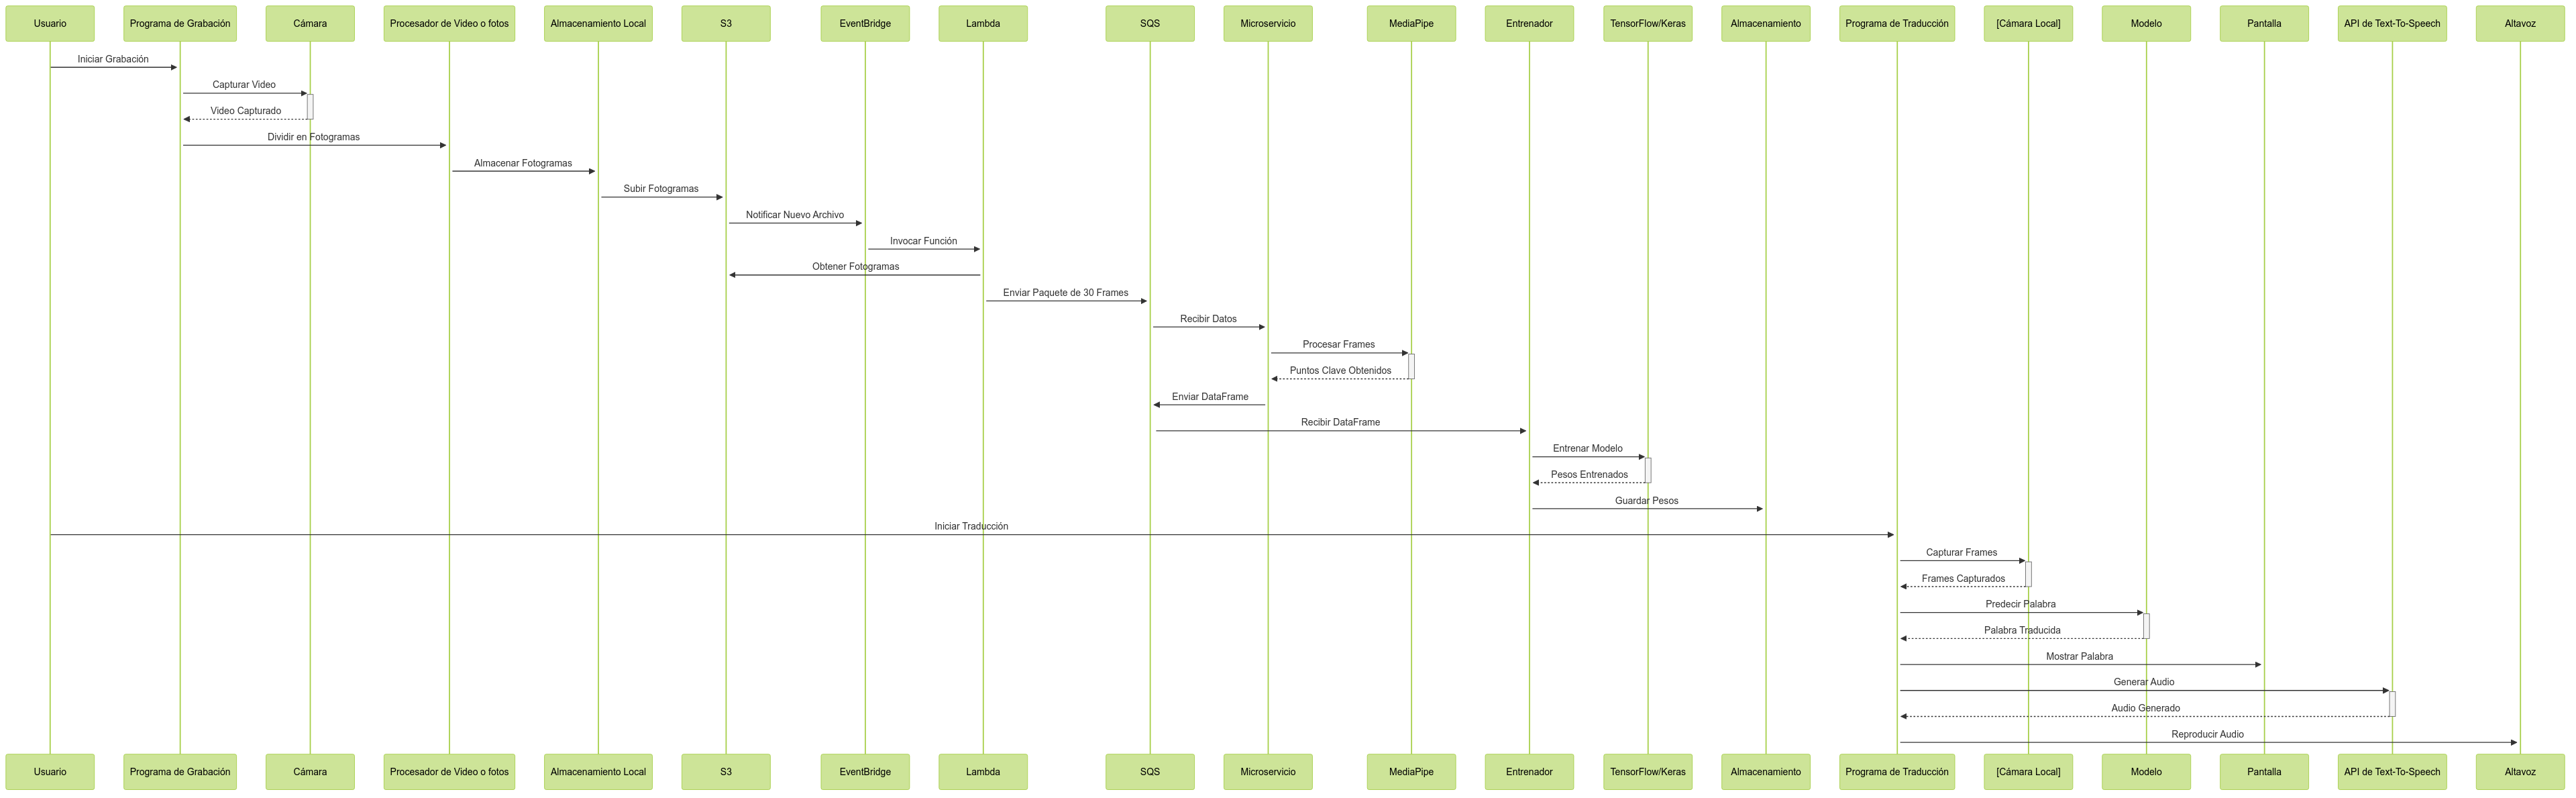
\includegraphics[scale=0.17]{CAPITULOS/capitulo1/digramacap1.png}
  \end{sideways}
  \centering
  \caption[Diagrama del funcionamiento del sistema]{Diagrama del funcionamiento del sistema}
  \label{fig:diagrama_sistema}
\end{figure}



\clearpage


\section{Alcances y limitaciones}


En resumen, los resultados que se esperan ser obtenidos son los siguientes:

\begin{itemize}
    \item \textbf{Reconocimiento de Señas Estáticas:} El sistema se enfocará en el reconocimiento preciso de un conjunto predefinido de señas estáticas de detención dentro de la Lengua de Señas Mexicana (LSM).
    \item \textbf{Ambiente Controlado:} El sistema funcionará de manera óptima en un ambiente interior sin incidencia directa de luz solar, para garantizar la calidad de la captura de imágenes por la cámara y la API de hand tracking.
    \item \textbf{Configuraciones Manuales:} Se deberá contar con configuraciones manuales otorgadas por la API de hand tracking, las cuales constituyen una característica importante, como la posición de manos y los dedos.
    \item \textbf{Señas de Convención:} Existe una similitud léxica alrededor del país de 80\% a 90\%, esto quiere decir que existe una variación dialectal, de acuerdo con la región del país, lo que se buscará es solo utilizar señas como convención por la mayoría de sordos \cite{ref22}.
    \item \textbf{Reconocimiento de Manos y Muñeca:} El sistema se limitará al reconocimiento de manos y muñeca, dentro del espectro permisible para la cámara y la API de hand tracking.
\end{itemize}

\section*{Limitaciones del Sistema}

Por el contrario, es pertinente mencionar lo que no se pretende con este sistema:

\begin{itemize}
    \item \textbf{No Reconocimiento de Frases o Textos:} El sistema no busca hacer reconocimiento de frases, o textos de mayor envergadura únicamente de palabras, dado a que la estructura gramatical de la LSM es muy diferente al español, cabe hacer mención que existe el español signado, pero no este no está dentro del enfoque en la problemática a solucionar \cite{ref21}.
    \item \textbf{No Deletreo:} Tampoco se busca hacer el reconocimiento de palabras por medio de deletreo, dado que ya existen sistemas que realizan esta tarea, de igual manera no representa una manera eficiente de expresarse.
\end{itemize}
\section{Justificación}

En México, el 33.5\% de las personas con discapacidad tiene una discapacidad auditiva y un 18\% presenta dificultades del habla, lo que significa que más del 51\% de este grupo se beneficiaría directamente de herramientas que faciliten la comunicación (Instituto Nacional de Estadística y Geografía \cite{ref1}. 
Para los miles de personas que dominan la Lengua de Señas Mexicana (LSM), este proyecto proporciona una plataforma que les permite transmitir mensajes a quienes no están familiarizados con esta lengua, enfatizando su importancia para la inclusión social \cite{ref16}.
Los estudios muestran que las personas con hipoacusia que tienen un nivel educativo más alto suelen tener un mayor dominio del español, debido a su acceso a recursos como libros e internet. Sin embargo, la falta de señas para ciertos conceptos limita su capacidad comunicativa, lo que a menudo lleva al uso del deletreo de señas en lugar del español signado.
Este trabajo busca desarrollar un sistema de diccionario de palabras en LSM que permita la traducción de señas a palabras en español, apoyado por la tecnología actual \cite{ref17}. Los diccionarios no solo proveen información lingüística, sino que también desempeñan funciones sociales significativas, como fomentar la identidad cultural y cohesionar a la comunidad \cite{ref18}.
La función primordial y más conocida de un diccionario es proveer información sobre una lengua, un diccionario además conlleva otras funciones sociales como dar identidad, función histórica y cohesión de la sociedad \cite{ref19}.
\section{Metodologia}
Para el desarrollo de este sistema de reconocimiento de LSM, se adoptó una metodología ágil inspirada en Scrum, la cual se basa en ciclos iterativos de desarrollo conocidos como sprints. Este enfoque, que prioriza la flexibilidad y la colaboración, se adapta de manera ideal a la naturaleza dinámica del proyecto, permitiendo la incorporación de mejoras y ajustes a lo largo del proceso. La adaptación de Scrum a este proyecto implica un enfoque iterativo en el desarrollo del sistema de reconocimiento de LSM. Se priorizarán las funcionalidades esenciales en los primeros sprints, como la captura y el procesamiento de las señas, y se irán incorporando nuevas funcionalidades, como la integración con la nube y la generación de audio, en sprints posteriores.

Este enfoque se inspira en la práctica descrita por Kniberg (2007), quien destaca varios principios clave de Scrum que aplican directamente a este proyecto\cite{ref39}:

\begin{itemize}
    \item \textbf{Enfoque en la práctica}: Scrum se centra en la aplicación práctica, lo que permite que el equipo se adapte a las necesidades del proyecto de manera eficiente.
    \item \textbf{Adaptabilidad}: La metodología se ajusta al contexto específico del proyecto, permitiendo mayor flexibilidad en lugar de seguir un conjunto rígido de reglas.
    \item \textbf{Colaboración}: La comunicación y colaboración entre el equipo de desarrollo y el Dueño de Producto son esenciales, especialmente durante la planificación de cada sprint.
    \item \textbf{Entrega continua}: Al final de cada sprint, se promueve la entrega de software funcional, asegurando que el producto esté en constante evolución y mejora.
    \item \textbf{Mejora continua}: A través de retrospectivas, el equipo analiza y mejora su proceso en cada sprint.
    \item \textbf{Simplicidad}: El proyecto se gestiona de manera simple, utilizando herramientas como tarjetas físicas para la organización del backlog del producto y del sprint.
    \item \textbf{Transparencia}: La transparencia en el progreso es fundamental, y se asegura mediante un tablón de tareas visible para todo el equipo y una página de información del sprint para mantener informada a toda la organización.
\end{itemize}
En la \ref{fig:imagen_scrum} se presenta un esquema de las etapas que conforman la metodología SCRUM:

\begin{figure}[h]
  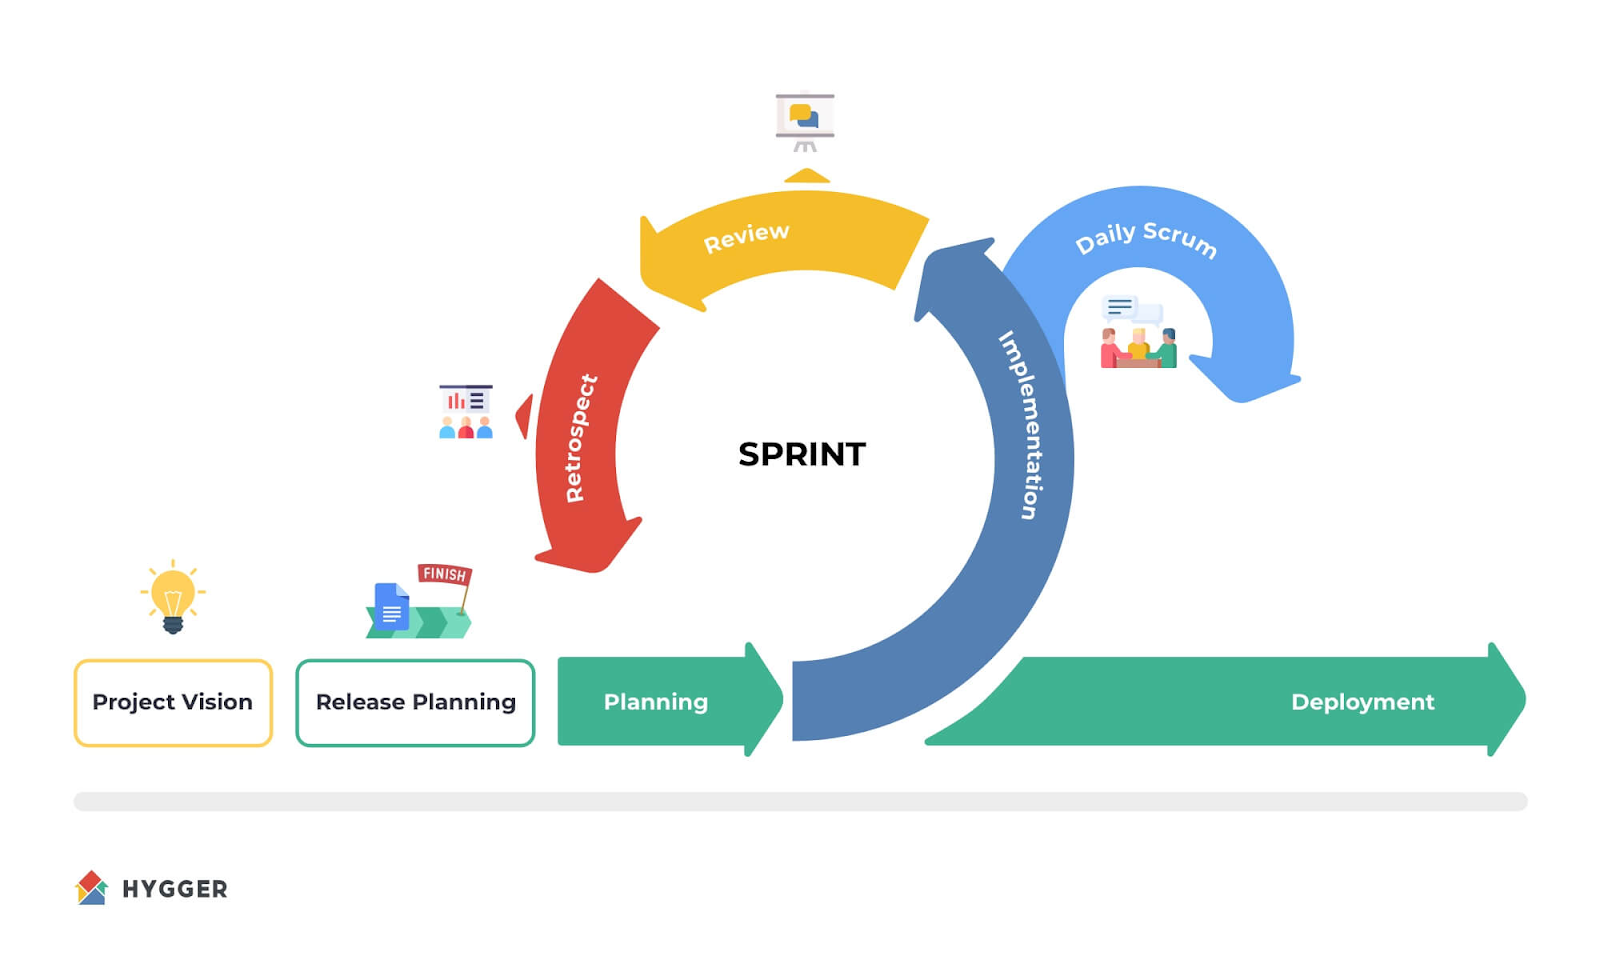
\includegraphics[scale=0.17]{CAPITULOS/capitulo1/scrum.png}
  \centering
  \caption[Metodología Scrum ]{Metodología Scrum \cite{ref40}}
  \label{fig:imagen_scrum}
\end{figure}

\clearpage

\section{Objetivos}

\subsection{Objetivo general}

Desarrollar un sistema de reconocimiento de señas estáticas de la LSM, con una arquitectura híbrida que combine componentes \textit{on-premise} y en la nube. Se utilizará MediaPipe u otra API de \textit{hand tracking} para la captura y procesamiento de datos, enfocándose en señas de configuración manual o de reposo y parametrizando las principales articulaciones manuales en un sistema de coordenadas rectangulares. A partir de estos datos, se entrenará un modelo de clasificación utilizando TensorFlow para reconocer y asociar las señas a su equivalente en español. La palabra reconocida será reproducida utilizando una API de voz (\textit{speech-to-text}).

\subsection{Objetivos específicos}

\begin{enumerate}
    \item \textbf{Recopilación de Datos:}
        \begin{itemize}
            \item Recopilar un conjunto de datos representativo de señas estáticas de detención en LSM, incluyendo variaciones dialectales comunes, y etiquetarlas con su significado en español.
            \item Utilizar una cámara web para capturar de las señas, asegurando una calidad adecuada en un ambiente controlado. Extraer una secuencia de fotogramas representativa de cada seña para su posterior procesamiento.
            \item Utilizar MediaPipe para extraer los puntos clave de las articulaciones de las manos en un sistema de coordenadas rectangulares.
        \end{itemize}

    \item \textbf{Modelado y Entrenamiento:}
        \begin{itemize}
            \item Seleccionar y adaptar un modelo de reconocimiento existente, como una red neuronal convolucional (CNN), para el reconocimiento de señas estáticas \cite{ref7}.
            \item Entrenar un modelo de reconocimiento de señas utilizando técnicas de aprendizaje automático (TensorFlow/Keras) con los datos recopilados y etiquetados.
        \end{itemize}

    \item \textbf{Diseño del Almacenamiento de Datos:}
        \begin{itemize}
            \item Diseñar e implementar una estructura de almacenamiento eficiente que combine una base de datos y un \textit{bucket} (como S3) para gestionar la información recopilada. La base de datos almacenará metadatos de las señas (traducciones, parámetros de articulaciones, configuraciones manuales), mientras que el \textit{bucket} almacenará las imágenes de las señas. Se asegurará la integridad de los datos y se facilitará el acceso a ambos tipos de información para el entrenamiento, la ejecución y el mantenimiento del sistema.
        \end{itemize}

    \item \textbf{Desarrollo de la Salida y Configuración:}
        \begin{itemize}
            \item Implementar un mecanismo de salida claro y accesible para presentar la traducción de la seña reconocida, ya sea en texto, audio (utilizando una API de \textit{Text-To-Speech}) o ambos, según los requisitos del usuario final.
            \item Considerar la posibilidad de desarrollar una interfaz web intuitiva para interactuar con el sistema, si los recursos y el alcance del proyecto lo permiten.
        \end{itemize}
\end{enumerate}